\chapter{Event reconstruction}

\intro{The reconstruction of basic analysis objects within an event is described. A key ingredient in the \gls{cms} reconstruction is the particle flow algorithm which forms particle candidates by combining various subdetector information leading to an improved spatial resolution and energy measurement. The focus is set on the reconstruction and performance of muons, electrons, jets, and the missing transverse energy in 8 and 13~TeV pp~collision data which are the input objects in this thesis to study single top quark production.}

The event reconstruction attempts to build and identify basic analysis objects from the raw detector data. In \gls{cms}, basic objects are particle tracks and vertices as well as charged lepton, photon, and jet candidates. During the reconstruction additional information such as the missing transverse energy, $\met$, and the likelihood of jets to originate from the hadronization of b~quarks~(``b-tagging'') is determined. Since $\tau$ leptons have not been utilized and photons are not relevant in this study of $t$-channel single top quark production a description of their reconstruction and performance is omitted here yet details can be found in Refs.~\cite{Khachatryan:2015dfa,Khachatryan:2015iwa}.


%##############################################
\section{Track reconstruction}
%##############################################

The track reconstruction from hits in the inner tracking system is split in two steps. First, in the local reconstruction, hits from charge distributions on the pixel and strip modules of the tracker are formed. Then, in the global reconstruction, trajectory candidates are first seeded and then sequentially build from hits. A curved track is fitted to the hits of trajectory candidates to estimates parameters like the particle's momentum and charge. The individual steps are described briefly in the following. More details can be found in Ref.~\cite{Chatrchyan:2014fea}.

Different algorithms are used to determine the local position of two-dimensional (one-dimensional) hits from the distributions of charge deposits on the pixel (strip) modules respectively. A fast estimation of the hit position is performed for pixel hits first whose outcome is utilized in the trajectory seeding and building stage only. Here, the 2D charge distributions are projected onto each axis. Then the positions are estimated from the charge at the edges of the charge distribution clusters while accounting for the Lorentz-drift in the modules. During the track-fit the optimal pixel hit positions are instead estimated by comparing the charge distributions against simulated templates for various incident angles~\cite{Swartz:2007zz}. In the barrel layers, the pixel hit resolution is measured as $9.4~\upmu\mathrm{m}$ in $\mathrm{r}\phi$ and ranges between $21\range45~\upmu\mathrm{m}$ along the z-axis depending on the incident angle~\cite{Chatrchyan:2014fea}. 

For the strips, charge clusters are formed if the channel readout of adjacent strips is sufficiently above their individual noise levels. The hit position is then calculated as a charge-weighted average over a cluster and corrected for the Lorentz drift and potential inefficiencies occurring at the edges of a module. The hit resolution depends on the cluster size and pitch of the modules. It ranges roughly between $10\range30~\upmu\mathrm{m}$ ($10\range50~\upmu\mathrm{m}$) for the \gls{tib} (\gls{tob}) modules respectively~\cite{Chatrchyan:2014fea}.

Track reconstruction is performed in multiple passes, called iterations, over the reconstructed hits to reduce the combinatorial complexity. Each iteration consists of the same algorithmic steps~(seeding, trajectory finding, track fitting, and selection) but is configured differently. The first iterations attempt to reconstruct only simple tracks which originate close to the interaction region and have a sufficiently large transverse momentum. The hits belonging to successfully reconstructed tracks are masked in subsequent iterations which reduces the combinatorics. Later iterations focus then on displaced or low momentum tracks which may not originate from the interaction region using the remaining hits. Figure~\ref{fig:reconstruction-trackingiter} shows the efficiency and acceptance for successfully reconstructing a track\footnote{Tracks are reconstructed ``successfully'' if at least 75\% of their hits can be associated to a simulated particle.} in simulation, broken down per iteration, as a function of its transverse momentum or displacement.

\myfigure{\label{fig:reconstruction-trackingiter}Efficiency and acceptance of successfully reconstructing a track in simulation per tracking iteration as a function of (a)~the transverse momentum and (b)~the transverse displacement. The figures are taken from Ref.~\cite{trackingpublic}.}{
\subfloat[]{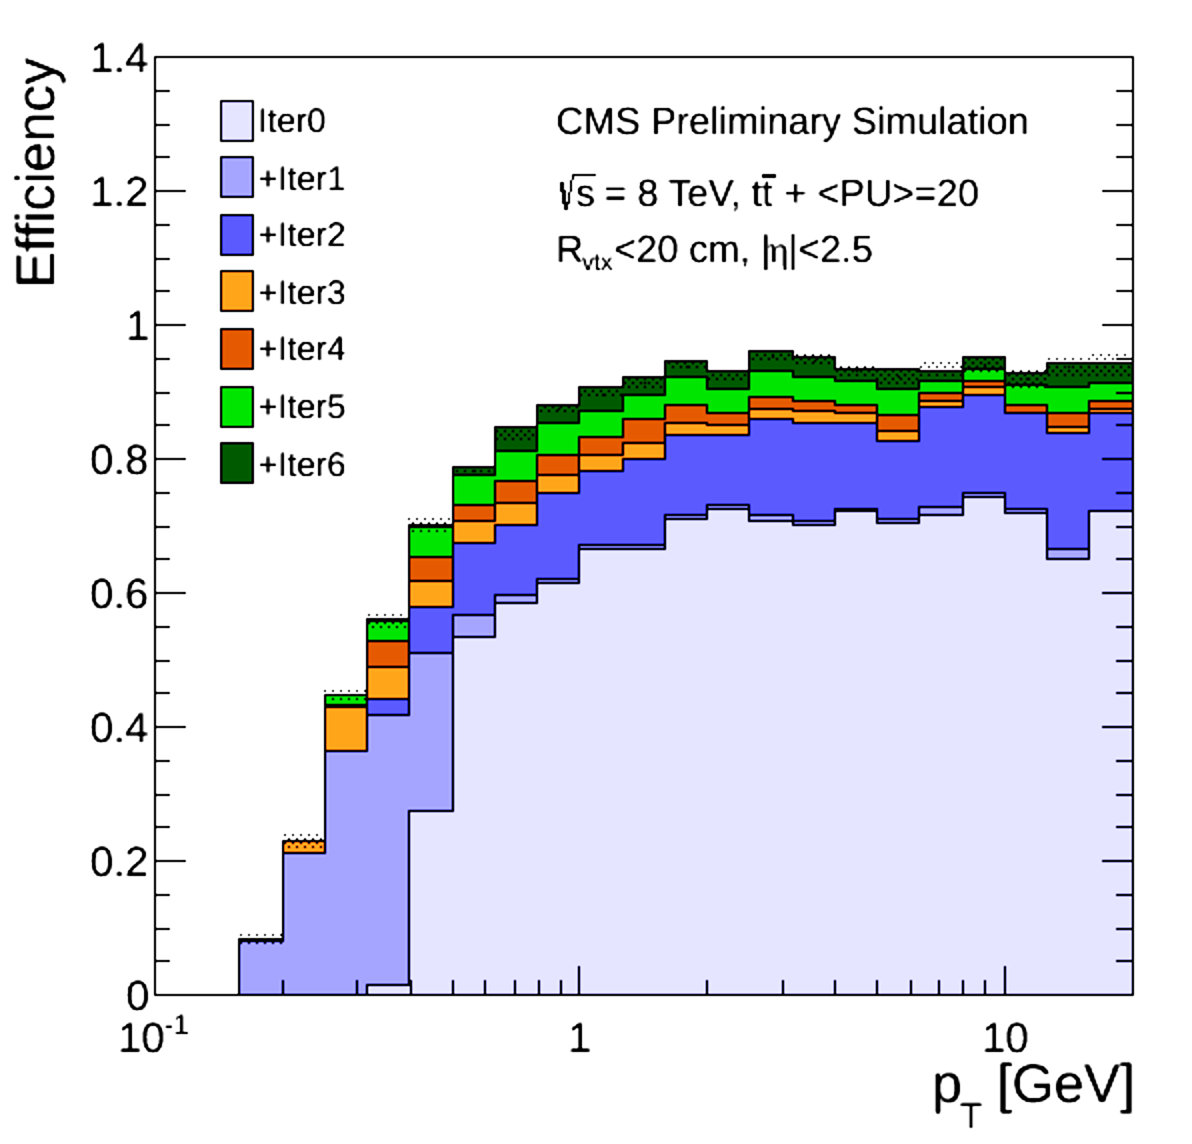
\includegraphics[width=0.48\textwidth]{figures/reconstruction/tracking_vs_pt.jpg}}\hspace{0.03\textwidth}
\subfloat[]{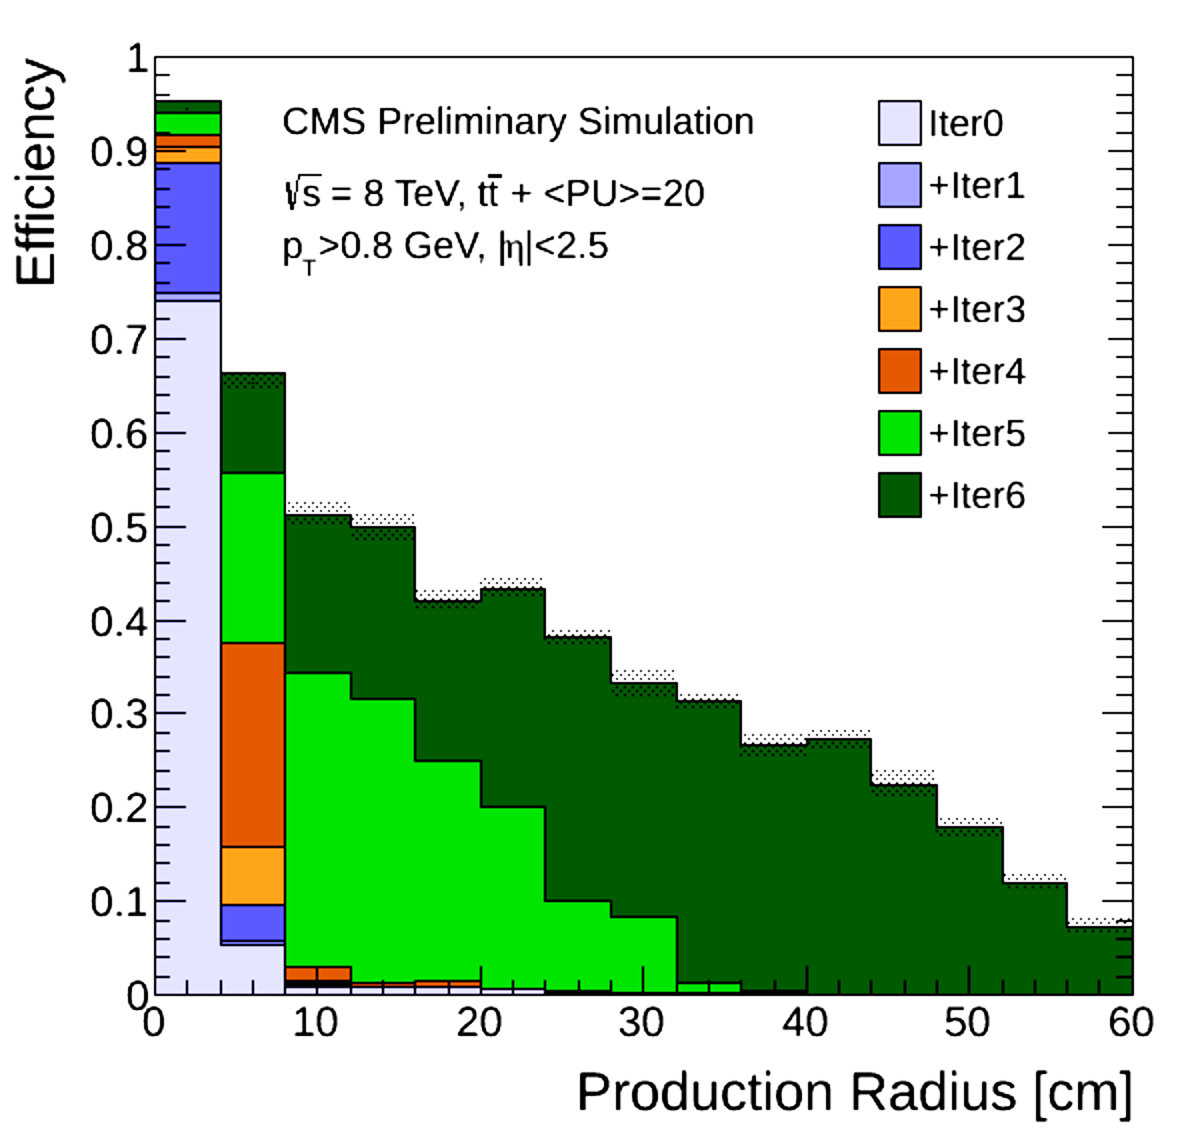
\includegraphics[width=0.48\textwidth]{figures/reconstruction/tracking_vs_vertpos.jpg}}
}

A trajectory seed is formed from a hit doublet or triplet where only certain combinations of tracker layers depending on the iteration are allowed for the hits. First iterations utilize mostly 3D hits on the pixel layers for seeding since their low channel occupancy results in less ambiguity and a higher efficiency for close-by tracks. Late iterations use hits on the strips instead where the spatial track density is low. Here 3D matched hits are utilized mostly which stem from double-sided strip modules but also mono layers are allowed. A seed candidate has to fulfill certain quality criteria depending on the iteration such as a minimal transverse momentum and compatibility with either the beam spot or a preliminary reconstructed vertex.

Each seed contains enough information to commence a first estimate of the track parameters. An algorithm called \gls{ctf} extrapolates the trajectory to find additional hits on subsequent layers which are compatible with the track hypothesis. It is based on the \gls{kf} technique which describes how to update the track parameters and their uncertainties iteratively after adding a hit. If multiple hits are found to be compatible with the track, new trajectories are generated for each of them. In the case no compatible hit is found on a layer a ghost hit is created instead.

The hits per trajectory are then passed to a \gls{kf}-based track fit to estimate the track parameters without utilizing the initial estimate from the seed. In addition, the fit accounts for material effects and the inhomogeneous magnetic field.  The fitted tracks have to pass a quality selection to reduce the amount of fake tracks before they are considered in physics analyses. The criteria reflect the seed requirements and depend additionally on e.g. the total number of (3D) hits, the $\chi^2/\mathrm{\gls{ndof}}$ of the fit, the amount of ghost hits, and the amount of shared hits with other tracks amongst others.

The tracking efficiency for isolated muon tracks with $1<\pt<100~\GeV$ is found to be above $99\%$ over the full tracker acceptance since their trajectories are only disturbed by energy loss through ionization and Coulomb scattering. The trajectories of charged hadrons like pions is additionally affected by nuclear interactions especially at low momenta ($\pt<700~\MeV$) which yields efficiencies between $80\range95\%$~\cite{Chatrchyan:2014fea}. For electrons, a special tracking is performed on top of the standard one which attempts to recover cases where the electron looses sufficient amounts of energy via bremsstrahlung as described in Sec.~\ref{sec:reconstruction-electrontracks}. In parts of the 2016 collision data the overall tracking efficiency decreased by about $2\range6\%$ at high instantaneous luminosities of $(1.0\range1.2)\cdot10^{34}~\mathrm{cm}^{-2}\mathrm{s}^{-1}$ due to a charge saturation effect on the readout chips leading to missing hits which was however recovered by adjusting the tracker module's charge drain speed.

%##############################################
\subsection{Muon tracks}
%##############################################
\label{sec:reconstruction-muontracks}

The track reconstruction for muons begins with the local reconstruction of hits in the three muon systems~\cite{Bayatian:922757}. The \gls{dt} hit positions are reconstructed by first forming independent segments in $r\text{-}\phi$ and $r\text{-}z$ through a combination of pattern recognition and linear fitting steps which are then combined. For the \glspl{csc}, independent 2D hits are reconstructed at wire-strip intersections in each of the six layers which are then combined to a track segment through a linear fit. Hits in the \gls{rpc} modules are build from clusters of fired strips where the positions are taken as the center of gravity of the cluster's area.

Standalone muon tracks are reconstruct from the information of the muon systems alone without utilizing the inner tracker. The tracking starts by generating seeds from a linear fit through hits in the \gls{dt} and \gls{csc} systems. Then, a \gls{kf}-based track-fit is carried out taking as starting point the seeds while also utilizing the hits in the \gls{rpc} system. In addition, the resulting track is constraint to be close to the beam spot which improves the momentum resolution. A region of interest inside the inner tracker is defined by extrapolating the standalone muon track inwards. A global muon trajectory is found and a track is fitted by utilizing also compatible hits from the inner tracker starting from trajectory seeds inside this region.


%##############################################
\subsection{Electron tracks}
%##############################################
\label{sec:reconstruction-electrontracks}

In \gls{cms}, the primary loss of energy for electrons occurs not via ionization but via bremsstrahlung instead. Typically an electron will radiate more than 70\% of its energy with a probability of 35\% in the tracker before reaching the \gls{ecal} leading to an increasingly curved trajectory in the magnetic field. Such trajectories are suboptimal to be reconstructed with the \gls{kf}-based standard tracking where a Gaussian-shaped energy loss distribution is assumed. Therefore, a different filter algorithm, the so-called \glshere{gsf}~\cite{0954-3899-31-9-N01} is employed instead.

Seeds for the \gls{gsf} tracking are constructed in two ways. The first method creates \gls{ecal}-driven seeds by forming super clusters of \gls{ecal} crystals with a size of 0.09 in $\eta$ but $\pm0.3~\mathrm{rad}$ azimuthally to detect electrons together with their potentially radiated photons~\cite{CMS:2010aua}. The second method tries to identify electron tracks inside the standard track collection which are typically marked either by a poor fit quality if the energy loss was large or that it is possible to match an \gls{ecal} cluster to the track otherwise. The resulting seeds from the two methods are selected to initiate the \gls{gsf} tracking. In its core it utilizes a set of trajectories which are subjected to the \gls{kf}-based tracking algorithm. For each trajectory a different Gaussian distribution for the energy loss through bremsstrahlung is assumed per layer. The summed distributions reflect an approximation of the Bethe-Heitler formula which describes the energy loss of electrons. After extrapolating the set of trajectories to a new layer, incompatible trajectories are removed or merged with similar ones to limit the exponential growth of trajectories to 12 at a time.

\todo{performance?}



%##############################################
\section{Vertex reconstruction}
%##############################################


The vertex reconstruction tries to locate points of pp interaction from which sets of charged-particle tracks originated. In analyses, this allows to separate the tracks from the hard scattering event from additional tracks belonging to pileup interactions. 

First, clusters of tracks are constructed using a deterministic annealing algorithm~\cite{726788}. For this only tracks which are close to the beam spot are selected. In the algorithm a statistical mechanics system is setup where each track reflects a microstate. The association of a track to a vertex candidate is floating and controlled by a probability. The free energy of the system is then monitored while decreasing its temperature. If a minimum of the free energy is reached a vertex is split in two nearby ones. The decrease of temperature is stopped when a trade-off between the expected resolution and the probability of falsely splitting two vertices is reached.

Finally, the vertex positions are estimated through an adaptive vertex fit~\cite{0954-3899-34-12-N01} per cluster of tracks. The obtained vertices are referred to as ``primary vertices'' since they mark the point of a pp interaction and are therefore lined up along the z-axis. The vertices are ordered by the summed $\pt^2$ of their associated tracks where the leading vertex is assigned to be the hard interaction of interest while the others are treated as pileup interactions. In 2016 pp collision data the primary vertex resolution is better than $\sigma_{z}=19~\upmu\mathrm{m}$ and $\sigma_{x,y}=14~\upmu\mathrm{m}$ for vertices whose summed \pt of associated tracks exceeds $100~\GeV$~\cite{CMS-DP-2016-041}.



%##############################################
\section{Particle flow}
%##############################################

A central element of the standard \gls{cms} reconstruction is the \glshere{pf} algorithm~\cite{CMS:2009nxa}. It combines the individual subdetector data to reconstruct global particle candidates like electrons, muons, photons, and charged and neutral hadrons in an event. By tracing the flow of particles through the various subdetectors an improved spatial resolution, energy measurement, and type identification of particles is achieved while avoiding double counting.

Its core consists of a linking algorithm which, given a particle hypothesis, links several subdetector information together. The linked elements can be charged-particle tracks from the inner tracker, calorimeter clusters from the \gls{ecal} or \gls{hcal}, and muon tracks. The algorithm starts by extrapolating charged-particle tracks into the calorimeter systems. In the \gls{ecal} the trajectories are extended to the expected depth of the shower maximum of an electron candidate. In the \gls{hcal} the trajectories are extrapolated up to one interaction length. A link is created if a trajectory is located inside the boundaries of a compatible \gls{ecal} or \gls{hcal} cell cluster within uncertainties. Photon candidates which could have been emitted tangentially from electron tracks are also created by extrapolating straight tracks from intersections of the electron track with the tracker layers to compatible \gls{ecal} cells. For neutral particle candidates, links between calorimeter clusters are formed. Here, the algorithm starts with \gls{ecal} or \gls{ps} clusters for which a good resolution is expected due to their granularity and extrapolates them to potential \gls{hcal} or \gls{ecal} clusters which have a coarser granularity respectively. A link between a tracker track and the muon system is created if the described track reconstruction for muons~(Sec.~\ref{sec:reconstruction-muontracks}) yields and acceptable goodness-of-fit.

The identification of particles is performed by utilizing the linked blocks. First, global \gls{pf} muons are identified if their momenta are compatible with the tracker-only track momenta. Then \gls{pf} electrons are identified through the \gls{gsf} tracking together with potential photons from bremsstrahlung. A \gls{pf} charged hadron candidate is created for each of the remaining \gls{pf} candidates that have a charged-particle track linked to it. Then, the amount of neutral energy is determined by subtracting the charged particle energy fraction from the calibrated energy of the linked calorimeter clusters. This procedure yields \gls{pf} photon and \gls{pf} neutral hadron candidates depending on the excess of neutral energy in the \gls{ecal} and \gls{hcal} clusters.

The improvement in spatial and energy resolution which is achieved through the \gls{pf} algorithm is demonstrated exemplary for jets in Fig.~\ref{fig:reconstruction-pfjets}. In particular, the energy resolution of \gls{pf} jets at low momenta is significantly better than that of calorimeter jets since here the energy estimation utilizes also the measured momenta of charged-particle tracks from the inner tracker.

\myfigure{\label{fig:reconstruction-pfjets}Comparison of simulated calorimeter and particle flow jets performance: (a)~spatial resolution in $\eta$; (b)~energy resolution. The figures are taken from Ref.~\cite{CMS:2009nxa}.}{
\subfloat[]{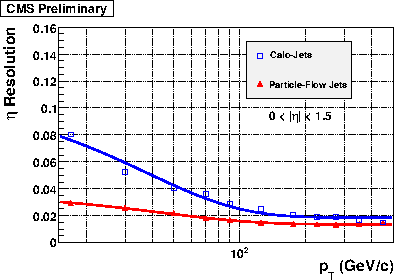
\includegraphics[width=0.48\textwidth]{figures/reconstruction/pf_jeteta.pdf}}\hspace{0.03\textwidth}
\subfloat[]{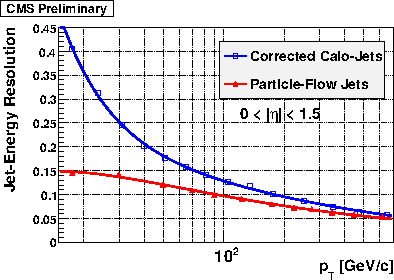
\includegraphics[width=0.48\textwidth]{figures/reconstruction/pf_jetenergy.pdf}}
}

%##############################################
\section{Muons}
%##############################################

Identification of muons for physics analyses is performed by requiring additional selection criteria. Different quality levels of muon identification allow to balance the purity against the efficiency. A description of various muon identification and  with 7~\TeV pp collision data can be found in Ref.~\cite{Chatrchyan:2012xi}.

Throughout the analyses within this thesis, the ``tight'' muon ID is used which attempts to selects the most genuine muons while rejecting falsely reconstructed one. The exact criteria defining tight muons are adapted slightly from one data taking period to the next. In the following, the details and performance of muon identification criteria utilized in 2012 pp collision data are briefly discussed.

Global \gls{pf} muons are considered for identification if they have a $\pt$ of at least $20~\GeV$ and fall within a pseudorapidity range of $|\eta|<2.1$. The global muon fit is required to included at least one valid hit in the muon chambers where two muon segments have to be present in at least two muon stations. This ensure that 

 To reject fake muons from hadron showers that are not contained by the \gls{hcal}, so-called ``punch-throughs'', 



\myfigure{\label{fig:reconstruction-idmuon}The figures are taken from Ref.~\cite{CMS-DP-2013-009}.}{
\subfloat[]{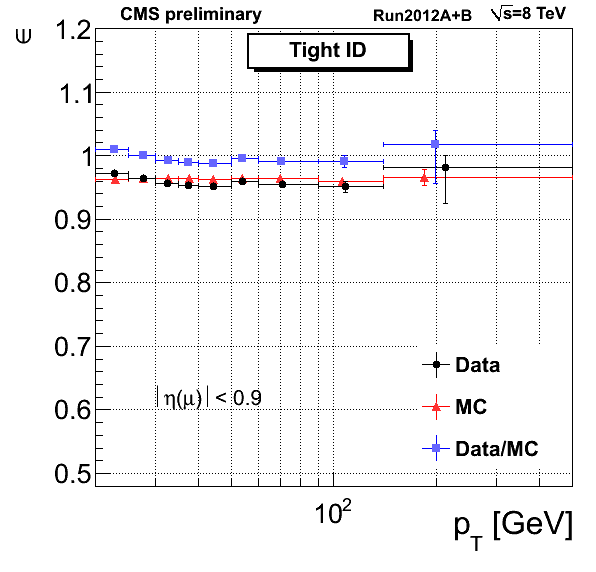
\includegraphics[width=0.48\textwidth]{figures/reconstruction/muon_idpt.png}}\hspace{0.03\textwidth}
\subfloat[]{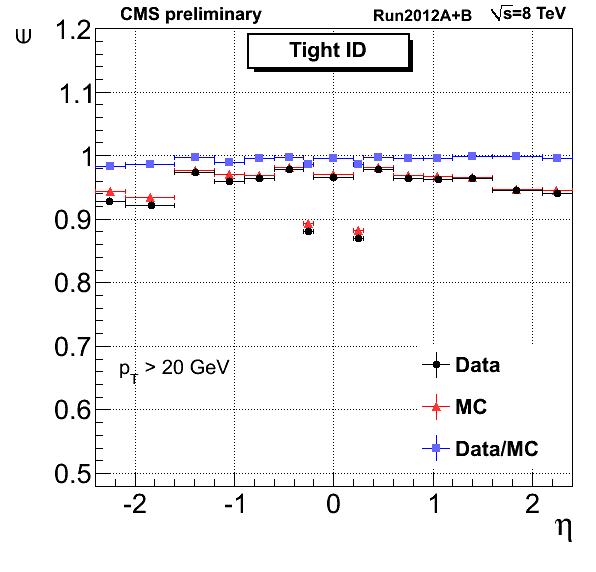
\includegraphics[width=0.48\textwidth]{figures/reconstruction/muon_ideta.png}}
}


\begin{equation}
I_\mathrm{rel.}^{\mu}=\frac{I_\text{ch.-had.}+\max\left(0,~I_{\gamma}+I_\text{neut.-had.}-\beta\cdot I_\text{\gls{pu}}\right)}{\pt^\mu},\qquad \beta=\frac{1}{2}
\end{equation}

\myfigure{\label{fig:reconstruction-isomuon}The figures are taken from Ref.~\cite{CMS-DP-2013-009}.}{
\subfloat[]{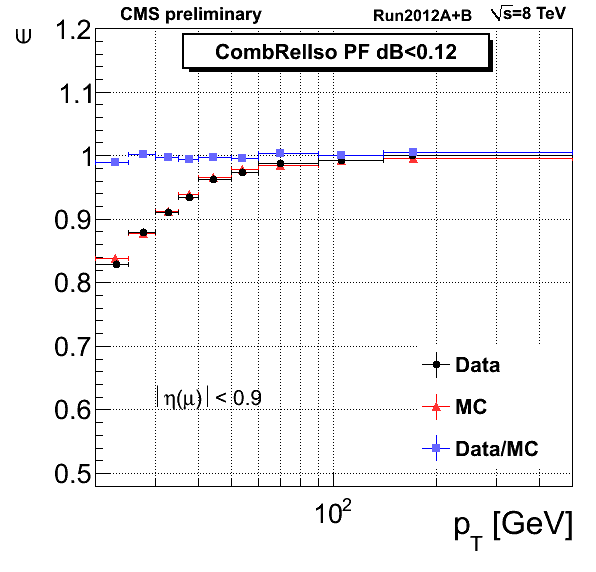
\includegraphics[width=0.48\textwidth]{figures/reconstruction/muon_isopt.png}}\hspace{0.03\textwidth}
\subfloat[]{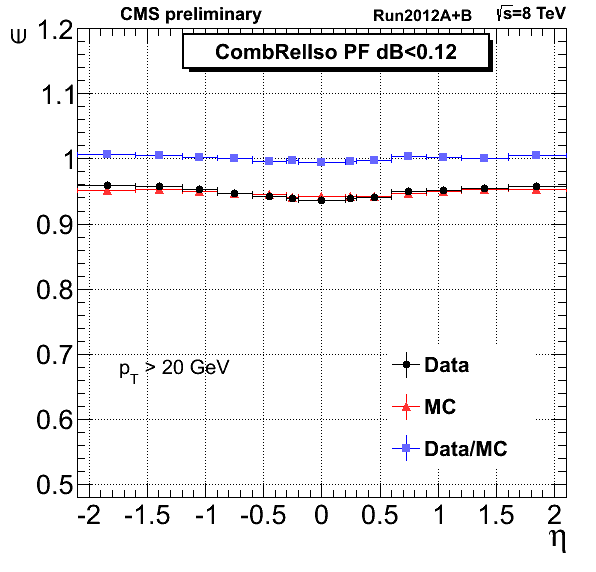
\includegraphics[width=0.48\textwidth]{figures/reconstruction/muon_isoeta.png}}
}




id, trigger

The relative 

%##############################################
\section{Electrons}
%##############################################
\label{sec:reconstruction-electrons}

id, scale factors, effective area isolation

\begin{equation}
I_\mathrm{rel.}^\mathrm{e}=\frac{I_\text{ch.-had.}+\max\left(0,~I_{\gamma}+I_\text{neut.-had.}-\rho\cdot A_\text{eff.}\right)}{\pt^\mathrm{e}}
\end{equation}

%##############################################
\section{Jets}
%##############################################

\myfigure{\label{fig:reconstruction-jets}The figures are taken from Ref.~\cite{CMS-DP-2013-033}.}{
\subfloat[]{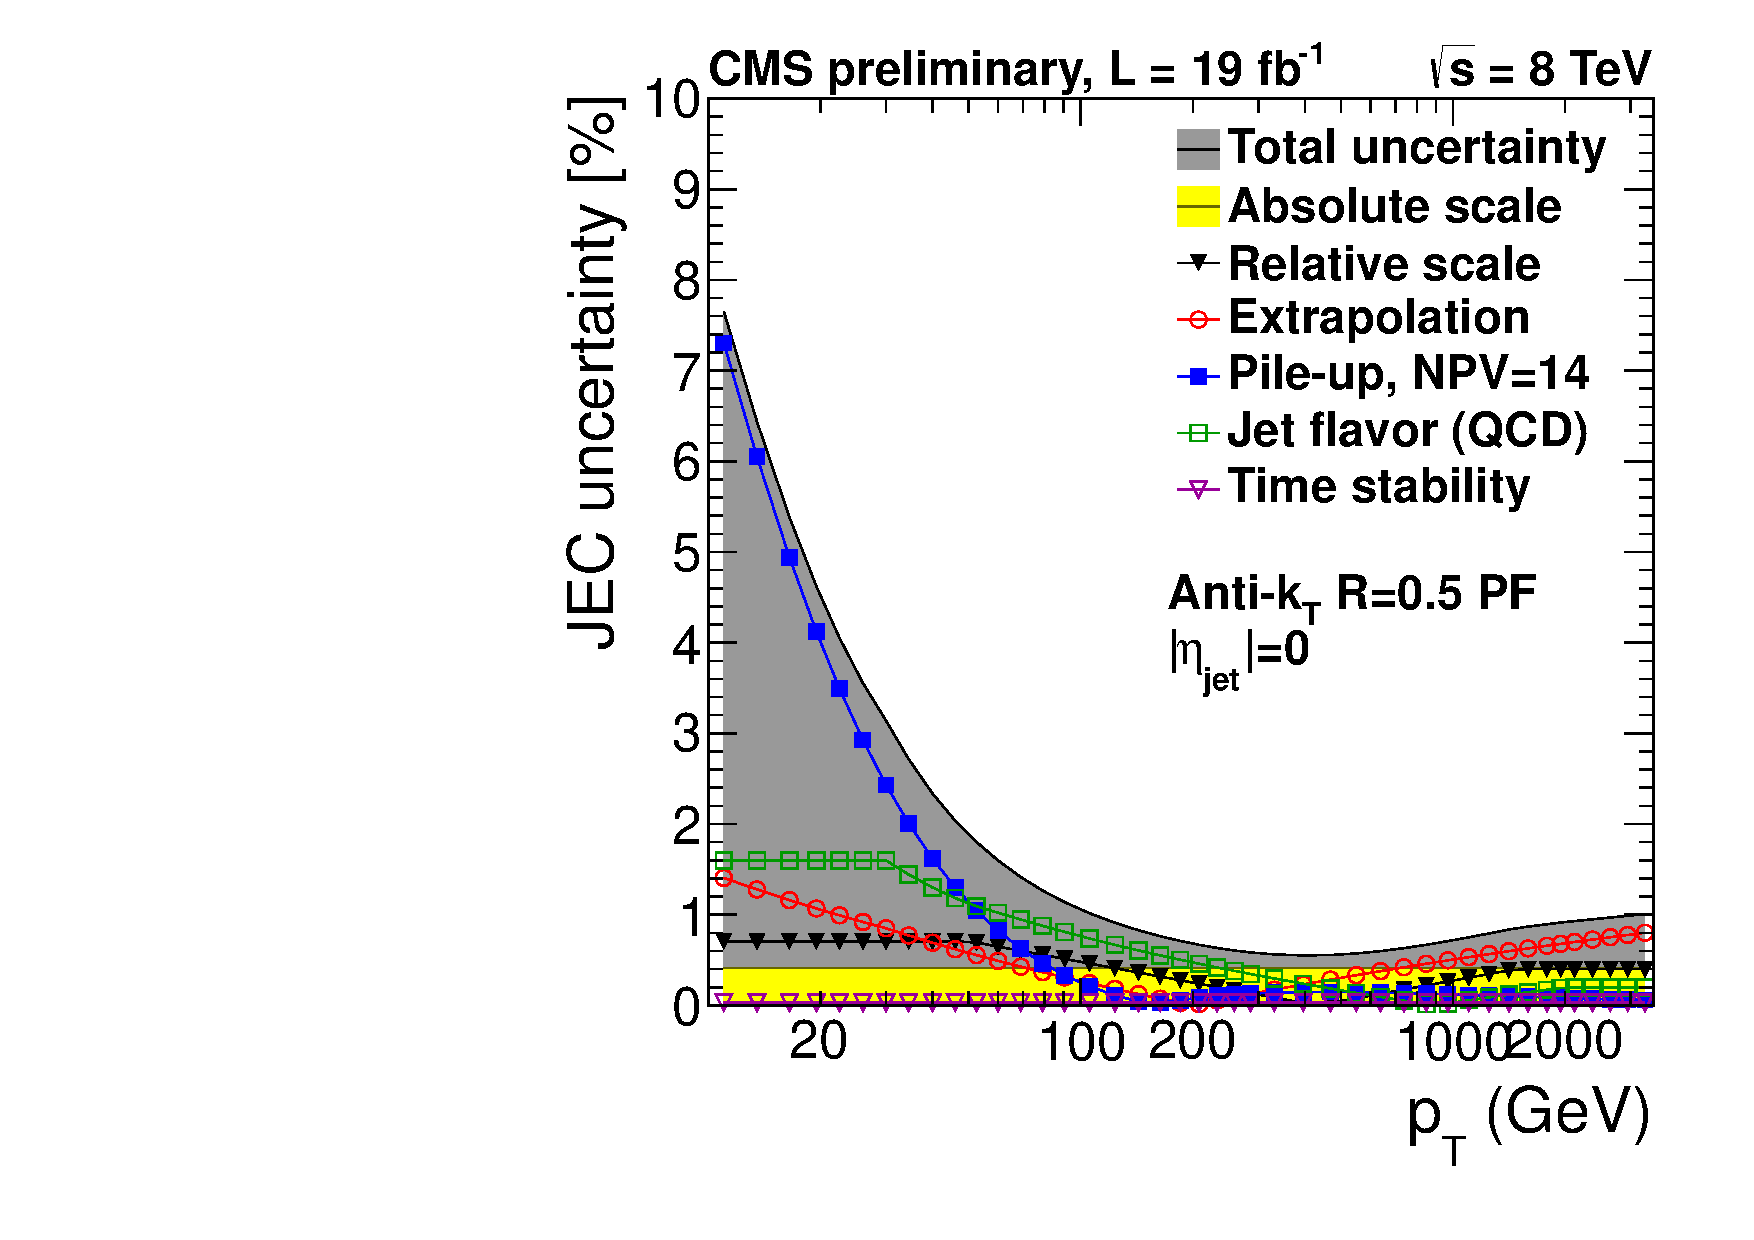
\includegraphics[width=0.48\textwidth]{figures/reconstruction/jet_uncpt.pdf}}\hspace{0.03\textwidth}
\subfloat[]{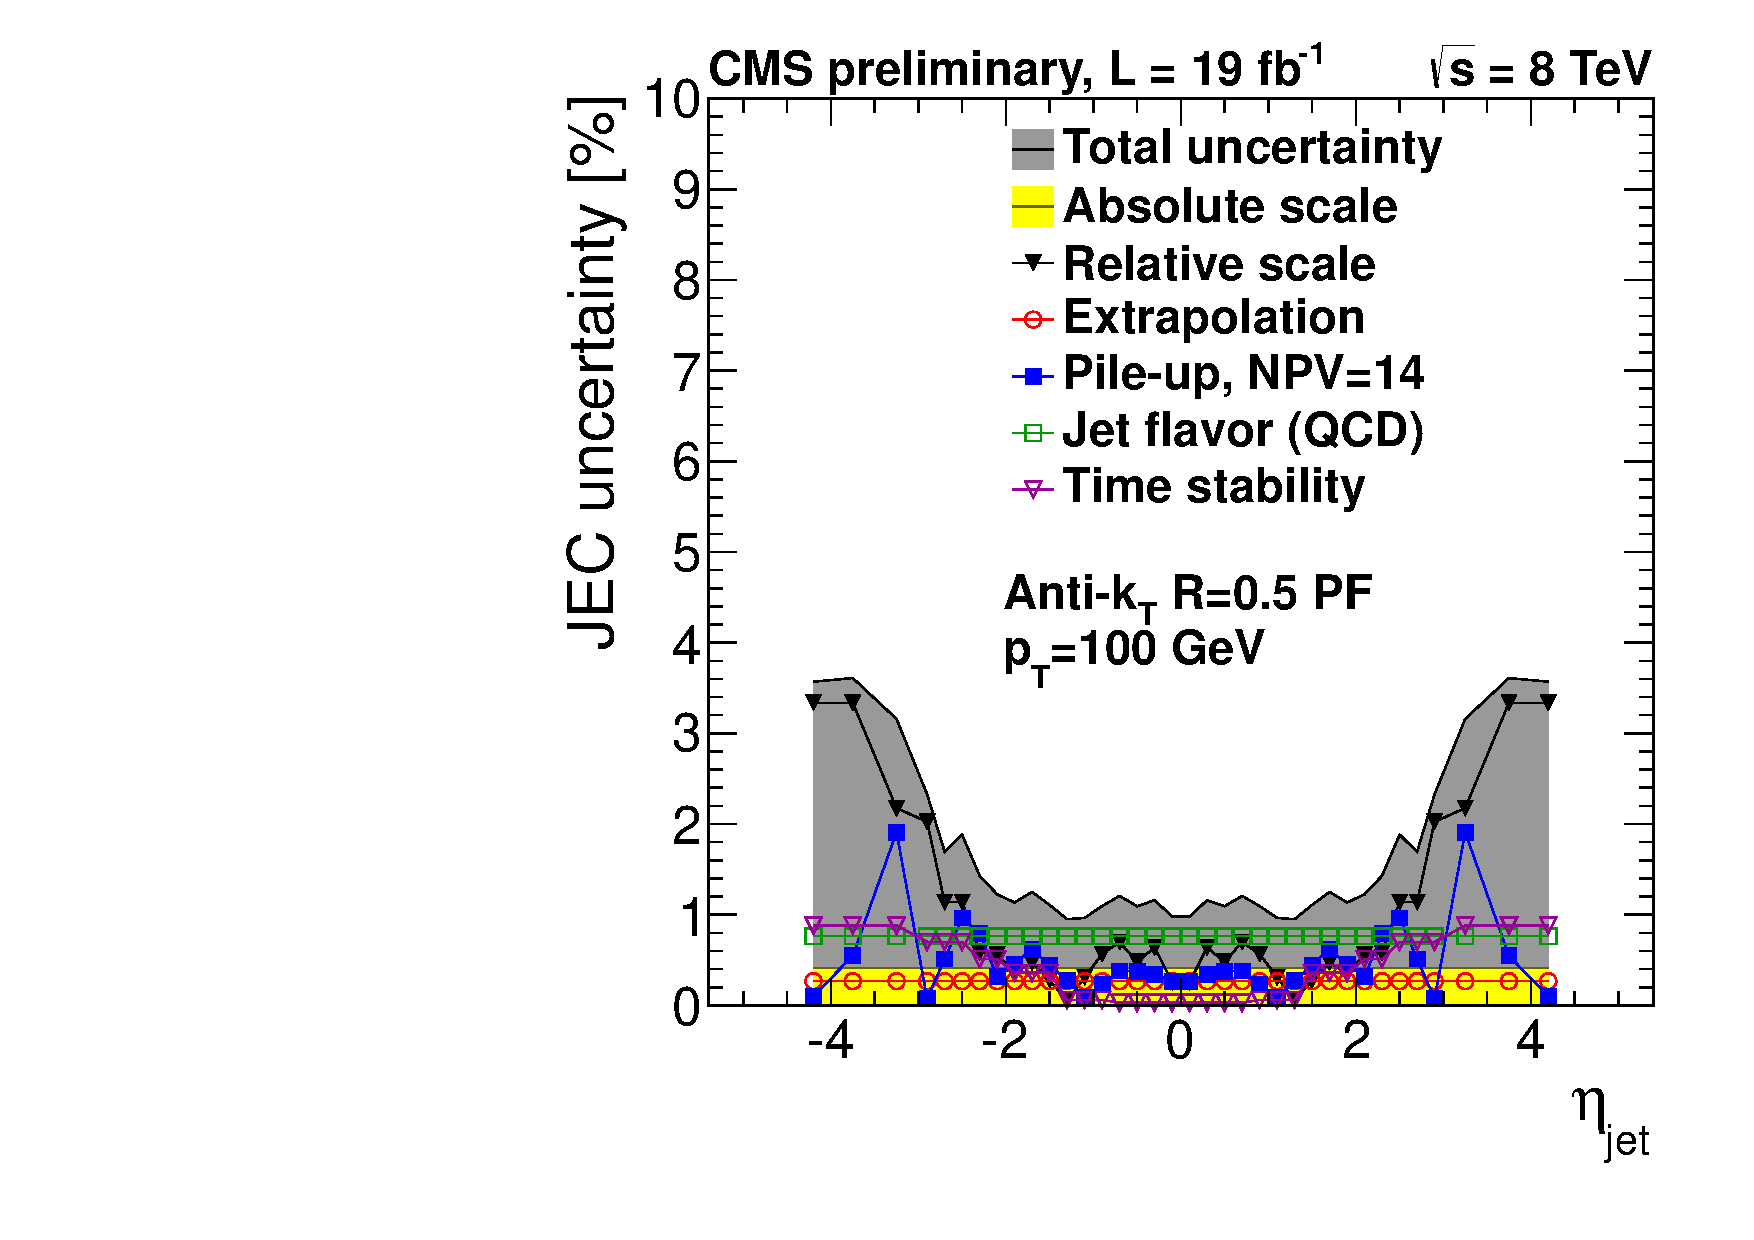
\includegraphics[width=0.48\textwidth]{figures/reconstruction/jet_unceta.pdf}}
}

hcal readout

ak clustering

leptob jet cleaning

CHS, JEC, JER

%##############################################
\section{b-tagging}
%##############################################

\myfigure{\label{fig:reconstruction-btagging}The figure is taken from Ref.~\cite{CMS-PAS-BTV-15-001}.}{
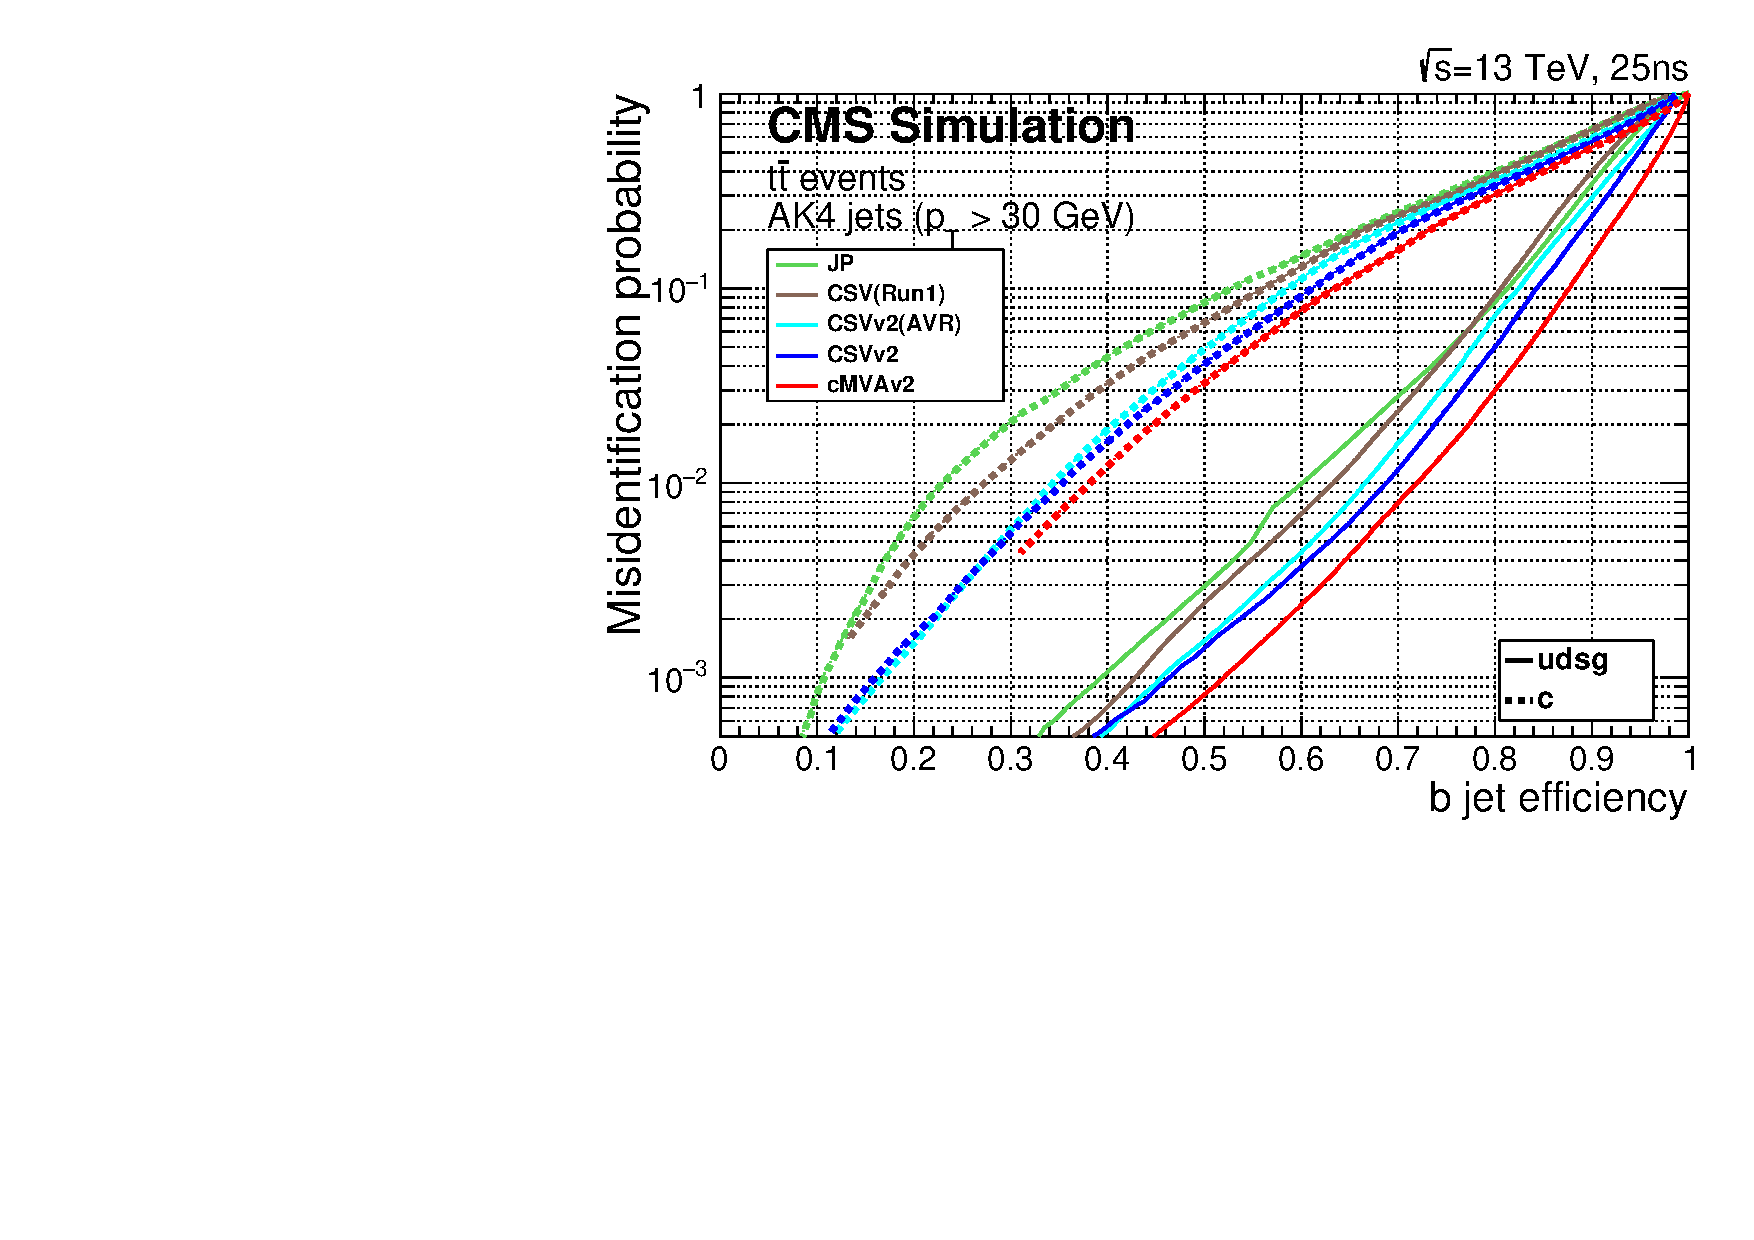
\includegraphics[width=0.75\textwidth]{figures/reconstruction/btag_comparison.pdf}
}

csv, SF, rizzi recipe

%##############################################
\section{Missing transverse energy}
%##############################################

for $\pt>50~\GeV$ the parallel $\pvmiss$ component is reconstructed well. At low momenta, unclustered energy degrades the 

\myfigure{\label{fig:reconstruction-met}The average $\pvmiss$ component parallel to the recoiling $\mathrm{Z}/\gamma$ boson as a function of the boson's momentum. The figure is taken from Ref.~\cite{CMS-PAS-JME-12-002}.}{
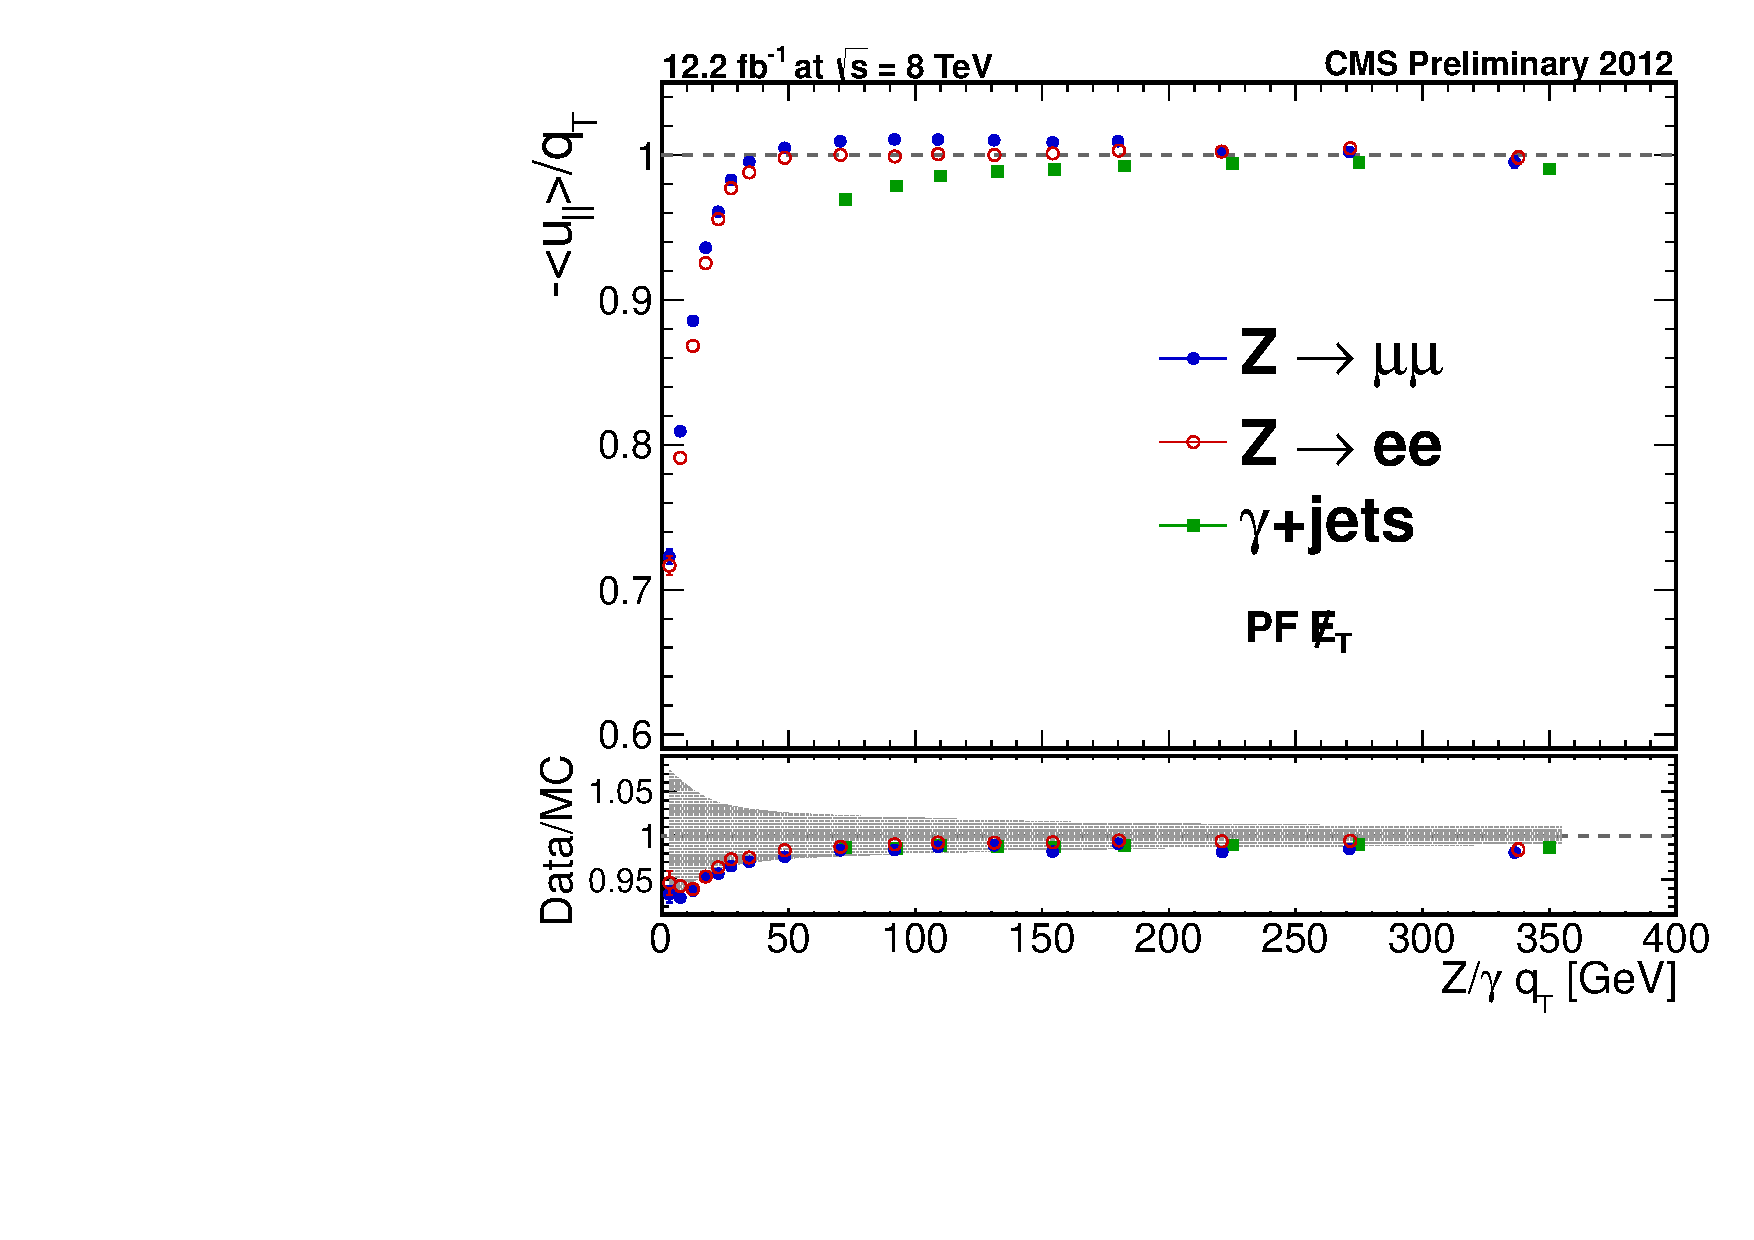
\includegraphics[width=0.6\textwidth]{figures/reconstruction/met_recoil.pdf}
}


T0, T1 corrections

%##############################################
\section{Luminosity and pileup}
%##############################################

pileup, rho
